\documentclass[
  utf8,%     More capable input encoding than latin-1.
  % parskip,%  For vertical whitespace between paragraphs.  This comes down to more than just using parskip.sty, so it's better to use this class option.
  % S5MP % If you intend to really use margin paragraphs (not recommended!).
%  crop,%     Produce output with crop marks and paper size A4.  Liu-Tryck should like this.  Automatically adds information, including the physical page number, at the top of each page.
       %     Add option 'noInfo' to suppress the info at the top of each page when using option 'crop'.
  % Font options: 'kp' (default), 'times', 'lm'.  The KpFonts (loaded using 'kp'), is the most complete font among the provided options.  Among other, it supports slanted small caps.  See rtthesis.cls for more details regarding the font options.
  largesmallcaps,widermath,% Good options to KpFonts.
  sharecounter,nobreak,definition=marks,%  See comments in the results chapter of this document for more information on these options!
  numbers, % If you want to cite references by numbers, use this option.
  noparts% Use option 'noparts' if you do not make use of part divisions.
]{rtthesis}

\usepackage{mythesis}

\begin{document}

\selectlanguage{english}
\makeFrontPage
\frontmatter
\maketitle
\makeLibraryPage{The number of connected devices connected to the Internet is growing rapidly, when talking about devices it also contains the once not having any contact with humans. This types of devices is the once that is expected growing the most. That is why the field of device fingerprinting is an area that which require more investigation. This thesis measure and evaluates the use of the accelerometer, camera and gyroscope sensors of a mobile device as fingerprinting of a device. The method used is based on previous research in sensor identification together with methods used for designing a biometric system. The combination with long-proven methods in the biometric area with new research of sensor identification is a new approach of looking at device fingerprinting.
}

\begin{abstract}[swedish]
  Sammanfattning är en sammanfattning på svenska...

\end{abstract}
\begin{abstract}[english]
  The number of connected devices connected to the Internet is growing rapidly, when talking about devices it also contains the once not having any contact with humans. This types of devices is the once that is expected growing the most. That is why the field of device fingerprinting is an area that which require more investigation. This thesis measure and evaluates the use of the accelerometer, camera and gyroscope sensors of a mobile device as fingerprinting of a device. The method used is based on previous research in sensor identification together with methods used for designing a biometric system. The combination with long-proven methods in the biometric area with new research of sensor identification is a new approach of looking at device fingerprinting.

\end{abstract}
\begin{acknowledgments}
I would like to thanks everyone that sending in the sensor data to my thesis, without you it would not be much to write about. Also many thanks to all employees at Cybercom, it has been fun working with the thesis when you were showing so much interest. Especially thanks to Dan Rosenqvist for all the good thoughts and ideas, and that I had the opportunity to work with this interesting topic. %Other persons at Cybercom I would like to thanks is of course my supervisor Philip Engström and contemporary thesis workers Felicia and Jessica.
\\
Other persons that have made my education to alot more fun than I expected is my classmate, 720 13-14 and LiU AIF IBK, love to all of you.\\
\\
The biggest acknowledgment goes of course to my parents who have always been there for me, without them I would never have taken me through this education. Then of course my brother Johan who is always with me.\\



  \addvspace{1em}
  \begin{flushright}
    \textit{%
      Linköping, June 2015\\
      Anna Karlsson%
    }
  \end{flushright}
\end{acknowledgments}

\tableofcontents
\begin{notation}% Passing the option "old" to the notation environment will redefine the notationtabular environment so that it produces an old style LaTeX tabular instead of a ctable.sty style tabular.
  \centering

  \begin{notationtabular}{Notation}{Notation}{Meaning}
    G\index{G!abbreviation} & G-force \\
    $\eta$ & \\
    $\epsilon$ & \\
    $\Theta$ & \\
    $\omega$ & \\
    $\boldsymbol{ F}_C$ & Coriolis force \\
  \end{notationtabular}

  \begin{notationtabular}{Abbreviations}{Abbreviation}{Meaning}
    FAR\index{FAR!abbreviation} & False Accept Rate \\
    FRR\index{FRR@!abbreviation} & False Reject Rate \\
    FTE\index{FTE!abbreviation} & Fail To Enrollment \\
    ICT\index{ICT@!abbreviation} & Information and Communication Technologies \\
    IoT\index{IoT@!abbreviation} & Internet of Things \\
    MEMS\index{MEMS!abbreviation} & Micro Electro-Mechanical System \\
    M2M\index{M2M!abbreviation} & Machine-to-machine \\
    NIC\index{NIC!abberviation} & Network Interface Card \\
    PRNU\index{PRNU!abberviation} & Photo-Response Non-Uniformity noise \\
    RFF\index{RFF!abbreviation} & Radio Frequency Fingerprinting \\
    RFID\index{RFID!abbreviation} & Radio-Frequency IDentification \\
    PRNU\index{PRNU!abbreviation} & Photo-Response Non-Uniformity noise \\
    FPN\index{FPN!abberviation} & Fixed Pattern Noise \\
    CFA\index{CFA!abberviation} & Color-Filter Array \\
  \end{notationtabular}
\end{notation}


\mainmatter
\chapter{INTRODUCTION}\label{cha:intro}
This paper is the report for my master thesis in Computer Science and the last part of my education of becoming an engineer in information-technology in the field of secure systems. The thesis was performed at Cybercom AB in Linköping. \\
This introduction chapter will give an overview of the work together with background and aims and objectives that is used as the basis for the work presented in this thesis. 

\section{Background}\label{sec:bg}
Cars, locks, birds, stoves, refrigerator, coffee maker, watches, cat feeder, sewing machines\dots, the world of connected devices is growing rapidly. This world is known under the term `Internet of Things'. For making this things connect to each other we need secure authentication methods for knowing that they are connecting to the device they are suppose to and not anything or anyone else. \\
\\
For us humans it has become an everyday thing to using two factor authentication when accessing buildings, part of networks, and our bank and so on. When talking about two factor authentication we usually use a combination of either three things; something you \textit{know} like passwords, something you \textit{have} like tag, passport, card, phone or something you \textit{are} like iris or fingerprint. (More about those in chapter ~\ref{cha:auth}.)  \\
Something you know or have is things that can be copied, stolen or modified fairly easy and without know all that much about the person or thing you try to authenticate as. This compared to something you are as iris, fingerprint and DNA requires much more effort and time since you can only focus on one person at a time. Machines or devices don't have those attributes as us human, they are build on hardware parts.\\ 
\\
The background of this thesis is to explore the possibility for a machine to have a fingerprint that can be used to more securely authenticate them. This can be applied in several areas for example in the new smart homes where fridges, stoves, coffee makers and doors should communicate with each other. Another example could be when you only want to limit the access to your bank account to your phone only to avoid that an malicious user accessing your account.

\section{Aims \& Objectives}\label{sec:aim}
Today most of the solutions for M2M authentication involves a certificate, token, UUID etc., this is something the machine know or have. The area of device fingerprinting has been more investigated in line with the world of connected devices that is called IoT (Internet of Things) has grown. The aim of this thesis is to look in to if the fingerprinting methods found today can be used as something the machine \textit{are} for two factor authentication between them. The problems this thesis aims to solve is:
\begin{itemize}
	\item[] Can you create a device fingerprint by using the sensor characteristics in a mobile device?
	\item[] Is this fingerprint suitable for using as a second factor for authentication between devices?
\end{itemize}
The problems above state a mobile device and not a general machine, which is one of the limitations in the thesis. The focus is also set to an authentication process where you are able to collect a set of data from the device in a database in an enrolment phase. This means that new devices in the system has to go through some phase were collecting the sensor characteristics, just like the police has to collect fingerprint from the suspect to compare with the fingerprints from the crime scene. As the title of the thesis implies, authentication is the focus not identification. As said in the background is a device building stone its hardware and something the devices \textit{has} that is the point of view of the thesis, similar to biometric authentication for us humans. \\
\\
The objectives of this work and can be summed up to:
\begin{itemize}
	\item[] \textbf{Explore different sensor characteristics of a mobile device} \\
	Mobile devices today are equipped with a lot of sensors and since they like other hardware has some bias that may be unique enough to differ from a device of the same model. Measurements from the gyroscope-, accelerometer- and camera-sensor will be collected and valuated like a biometric fingerprints.
	\item[] \textbf{Combining M2M, two factor and biometric authentication} \\
	Biometric authentication has ways of measure and compare fingerprints, this measurements and methods will be used to make the two factor authentication between the devices.
\end{itemize}

\section{Thesis Outline}\label{sec:outline}
This introduction chapter including background, aims and objectives will give a quick view of what the thesis is about. The chapters that following is divided in different parts that maps to the different objectives listed above.
\begin{itemize}
	\item[Ch.2:]	How authentication is made today between machines, two factor and in biometric.
	\item[Ch.3:]	The different hardware characteristics of a mobile device together with previously work in the area.
	\item[Ch.4:]	The method used when doing measurements of the characteristics described in chapter 3.
	\item[Ch.5:]	Result of the measurements.
	\item[Ch.6:]	Discussion about the result and method used with an discussion about the work in a wider context.
	\item[Ch.7:]	Conclusions that connect back to the aims and objectives and also includes further work of the thesis.
\end{itemize}
\chapter{COMMUNICATION \& AUTHENTICATION}\label{cha:auth} \index{authentication}
Since about all devices that are connected to a network are one way or another connected to the Internet you can bet that they find themselves in an untenanted or malicious environment. Everything connected to the Internet is very likely to be hacked. Thus, authentication is needed for remote sensing devices to communicate. \cite[]{auth:M2Mcom}\\
This chapter will present ways of authentication (two factor, M2M and biometric) that are in the area of this thesis. The section about biometric is included in the thesis because it has methods of measure strength of a biometric trait (especially fingerprint). These methods will be used when comparing strength of characteristic noise in the mobile device. \\


\section{Two factor authentication}\label{sec:2fauth} \index{two factor authentication}
There are more ways to authenticate a user than password, however it is the most common. There are three different types of authentication; 
\begin{itemize}
	\item Something the authenticator \textit{has} like a key, card, passport and so on
	\item Something the authenticator \textit{knows} for example password
	\item Something the authenticator \textit{is}, known as biometrics such as fingerprint or iris pattern
\end{itemize}
\cite[p.~31]{rosssec} \\
Authentication in two factor means a combination of two of the three types of authentication above. An example can be the use of a credit card (you have) in combination with a PIN-code (you know) to collect the money from an ATM. Something the authenticator has and knows is the most common combination. The biggest reason for that biometrics is not that common yet is due to costs.
\cite[p.~47]{rosssec}

\section{Challenge-Response authentication}\label{sec:challResp} \index{challenge-response}
The challenge-response protocol is built upon the idea that the user of a system first must complete a challenge decided by the system in order to access the system. An example is modern car keys when trying to start the engine, the engine controller gives the key a challenge consisting of a random $n$-bit number. The key encrypts the challenge and responds. \\
The problem challenge-response protocols faces is often to achieve good randomness, thus if the challenge is not random enough there is a risk for a malicious user to calculate the $n$-bit number. \\
There are other applications than locks, like the HTTP Digest Authentication. That uses the authentication process where a web server challenges a client or a proxy with the common secret of a password. The server sends nonce to the client or proxy, that hash the nonce with the password and the requested URI. (Nonce is an arbitrary number that only can be used once, often generated as random or pseudo-random.) This authentication mechanism is not vulnerable to password snooping and is used in cases like client-server-authentication in SIP or the protocol for Voice-Over-IP telephony. This protocol is vulnerable to man-in-the-middle attacks. \\
\\
Ross states that a much more common use of challenge response is in \textit{two-factor authentication} (\sectionref{sec:2fauth}). An example of use is if you have a bank card reader when accessing your bank on the Internet. When you want to log in there are a random set of $n$ numbers displayed in the screen. You put these numbers together with a PIN into your bank card reader. The reader encrypts these numbers (pin + $n$ numbers) using a secret key shard with the server of the bank. The first $n$ numbers of the encryption is displayed on the card reader and you enter this in the login screen as a password.
\newpage
\begin{figure}[h]
	\centering
    \includegraphics[scale=0.4]{img/challenge-response-bank}
    \caption{Challenge-response authentication with bank card reader}
  \label{fig:challengeResponse}
\end{figure}
Describe ~\figureref{fig:challengeResponse}:
\begin{enumerate}
	\item Bank sending challenge XXXX XXX to the requesting address.
	\item User enters PIN and XXX XXX in the bank card reader.
	\item The reader encrypts the PIN and number with a secret key shared with the bank. The first numbers of the encryption are displayed o the reader. ($YYYY YYY = {XXXX XXX, PIN}_k$) 
	\item The user enters the encrypted numbers YYYY YYY on the log in screen and sends it as a password to the bank.
\end{enumerate}
~\cite[ch.3]{rosssec}

\section{M2M\index{M2M} (Machine-to-machine)}\label{sec:m2mauth}
Information that is exchanged via a communication network between machines has to establish conditions for doing so, that is where M2M is used. M2M is often a short synonym for M2M communication, meaning the communication conditions between devices. M2M communication is only the communication made between machines without any human behind it. A mobile device interacting with a call center application is not M2M, because there is a human behind the mobile device calling. 
The reason for using mobile devices in this thesis, that is controlled by a human, is that they contain many sensors. These sensors can be found in other simpler devices where M2M communication can be applied.
\\
M2M often involves similar devices in the same M2M area network that are interacting with an application. This makes it possible for devices to access public networks as well, via a gateway or router. An example is the heating system in smart homes. 
The area of M2M are important to make these devises talk without a human behind. This affects the requirements on the applications and networks dealing with the devices. Characteristics of these devices are listed blow:
\begin{itemize}
	\item \textit{Multitude} - The part of IoT that not directly interacts with humans is the part growing the most. It is soon expected to be significant more than the ones which interact directly with humans. This will put more pressure on application and networks dealing with all devices.
	\item \textit{Variety} - The connected devices has requirements like data exchange rate, form factor, computing, or communication capabilities. M2M applications have to be built, in order to define and develop common enabling capabilities.
	\item \textit{Invisibility} -  Meaning that the device has virtually zero human control. The more invisibly the less likely for error caused by humans. 
	\item \textit{Criticality} - Devices that can harm humans like electrical errors. Therefore reliability is an important factor. 
	\item \textit{Intrusiveness} - Many of the increasing connected devices raise the privacy question like refrigerators, stoves, doors, etc.
\end{itemize}
All these devices with no human control is like told above very different, but many of them is similar in some ways, such that the functionality is limited, low-powered, embedded and have long life cycles. The fact that they often are embedded makes it hard to separate between M2M communication and machine-to-human or human-to-human communication.
\cite[p.~2-4]{m2mComm}

\subsection{Difference between M2M and IoT}\index{IoT}
The term Internet-of-Things meaning everything that is connected to the Internet. IoT are now in its starting pits and ready to start the race. Machine-to-machine communication is a part of that, but it also covers other areas and IoT some that M2M does not. 
% Måla en fin graf med två ringar som sitter ihop om du vill förklara.
The common denominator is according to Polsonetti the \textit{remote device access}, where the embedded hardware modules in a machine that communicate wireless or not is M2M applications. Remote device access for IoT has a wider perspective that not only including same device communication but also passive and other low-power sensors that not can be motivated as a M2M hardware module.
\cite[]{cpM2MIoT}

\subsection{M2M authentication}\index{M2M authentication}
There is no standardized way of authentication in M2M, but effort is done in the area. An example is authentication based on a machines fingerprint. (This fingerprint is not of the same character as the one this thesis.)  The fingerprint in the example  consist of hardware message of computers, such serial number of CPU, MAC address of network card, Machine ID etc. \cite[]{auth:M2M} \\
These things have through the years been proven to be pretty easy to spoof. There are hundreds of blog-articles and forum topics of how to do that in many platforms like mobile devices. \\
\\
Quote about M2M authentication:
\begin{center} 
\textit{``\dots traditional methods such as “what you know and who you are” may not be applied''.}
\end{center}
  \begin{flushright}\cite[]{auth:M2Mcom}\end{flushright}

This quote states pretty well the aim of this thesis (section~\ref{sec:aim}). That is to use what the device is with biometric authentication that is more  tried and tested.


\section{The biometric process}\label{sec:biometric}\index{biometric process}
\begin{center}\textit{``A biometric system measures one or more behavioral characteristics...information of an individual to determine or verify his identity.''} \end{center}\begin{flushright}\cite[p.~3]{introbio}\end{flushright}

\subsection{Recognition}
As said before is biometric something you \textit{are} and the person who wants to be recognised to the system. Buy, showing his or her biometric identifier (fingerprint, iris, DNA, etc.) to the biometric system, therefore seen as a \textit{user} of the system. The strength in biometrics is also the fact that it knows if a user is known to the system even if the user denies it. \cite[ch.~1]{introbio}

\subsection{Biometric systems}\label{sec:bioSys}
There are some blocks for building a biometric systems, which can measure characteristics of a user. In biometrics these characteristics are called \textit{traits, indicators, identifiers, or modalities}, but in thesis it will still be called characteristics.\\
\\
The first step of biometric authentication is to collect biometric data and store it in a database with the user’s identity. The recognition is then done by again collecting biometric data from the user and compare to the database. This is the so called \textit{enrollment and recognition phase}. The raw biometric data is often destroyed after enrollment and the recognition is all about pattern matching. This matching is done in four steps;
\begin{enumerate}
	\item \textit{Sensor -} to collect the raw biometric samples, that can be an image, amplitude signal, online signature, odour or chemical-based.
	\item \textit{Feature extractor -} Makes the raw biometric samples comparable, mostly done in three pre-process operations; 
	\begin{itemize}
    	\item Quality assessment - Checks if the sample is good enough.
		\item Segmentation - removes the background noise from sample.
		\item Enhancement - Uses an algorithm to improve characteristic features of the sample.
    \end{itemize}
	\item \textit{Database -} that has the data from the enrollment phase together with some identity data (like name or ID). This database should having an access control mechanism for security reasons.
	\item \textit{Matcher -} where the sample from the enrollment is compared with the sample in recognition, to see if it is a match or not. This is done by having a match score to decide how close the enrolled and recognition sample is. The score is counted in different way depending on the characteristics that is used in the system. 
\end{enumerate}
\cite[ch.~1]{introbio}

\subsection{Biometric authentication}\index{biometric authentication}
Biometric authentication, is sometimes also called verification that answers the question \textit{Are you the one you say you are?}. There is also biometric identification that answers \textit{Are you someone known to the system?} but that is not what this thesis aims to answer. The practical difference between authentication and identification is that the user has to give the system some kind of information (username, passport, email etc.) on who they claim to be. But in identification the user just gives the sample to the system, which then checks if the user is known to the system or not. The identification look-up takes longer time since it compares the biometric input with all samples in the database, authentication only compare with the claimed identity. \cite[ch.~1]{introbio}

\subsection{Biometric measurements}\label{sec:bio:measure}
Biometric measurements are a bit trickier than in a password-based system where the answer just is match or not match. The accuracy of the biometric system must be considered when choosing characteristics. This is measured by two rates FRR\index{FRR} (False Reject Rate) that is the probability that two samples from the same user is not a match and FAR\index{FAR} (False Accept Rate) is the probability that two samples from different users is a match. 
There are a threshold $\eta$ that is used to decide the FRR and FAR. The proportion of authentic scores ($\omega_{1})$) that are less than $\eta$ is defined as FRR and the impostor score ($\omega_{0})$) that are greater than or equal to $\eta$ is FAR. The rates can be described mathematical as;
$$ FAR(\eta) = p(s\geq \eta | \omega_{0}) = \int_{\eta}^{\infty} p(s | \omega_{0}) ds, $$
$$ FRR(\eta) = p(s\geq \eta | \omega_{1}) = \int_{-\infty}^{\eta} p(s | \omega_{1}) ds, $$
where $p(s\geq \eta | \omega_{x})$ us the probability density function of the authentic respective impostor score. 
\cite[p.~18]{introbio}

\subsection{The design of a biometric system}
When designing a biometric system it is done in an activity cycle of five steps. Depending on the outcome of one activity, the next step could be forward or redoing earlier activity. These five steps are explained below followed by an flow-chart of the design cycle.\\
\\
\textbf{Understand nature of application}\\
Deciding functionality upon type and classification based on how well the system fits this different behaviors; cooperative, overt, habituated users, attended, untenanted operation, controlled operation and open system. \\
The first is if the user will be \textit{cooperative} or not, like if the user wants to access something it is likely to cooperate. \textit{Overt} is if the user knows that it is object for biometric recognition. If the user interacts with the system a lot it is likely that the user will be \textit{habituated}. The enrollment and recognition operations can either be \textit{attended} by a human or not. The environment of the operations may have to be \textit{controlled} in terms of temperature, pressure, etc. in order to work. Last there is the question of if the system will be closed or \textit{open}, such if the database of biometric data will be shared between applications or be in one closed application.) \\
This chapter and the next that includes theory, can be compared to this part of the biometric design cycle.\\
\\
\textbf{Choose biometric characteristics }\label{auth:bio:character}\\ 
This choice is based on seven different factors. The disadvantages of biometrics is that it will never be completely solid, therefore factors will have different significance in different systems.
\begin{enumerate}
	\item \textit{Universality,} the fail-to-enrollment (FTE) rate should be low.\index{FTE}\index{universality}
	\item If the \textit{uniqueness} of the characteristics is high the rate of FAR will be low. \index{uniqueness}
	\item The characteristic should be high in terms of \textit{permanence} and not be changing significantly over time.\index{permanence}
	\item \textit{Measurability} from the user perspective in terms of collecting characteristics should be convenient.\index{measurability}
	\item The time of the authentication is measured in \textit{performance}.\index{performance}
	\item User should have a high \textit{acceptability} when presenting their characteristics to the system.\index{acceptability}
	\item \textit{Circumvention}, in terms of how easy it is to maliciously fake the characteristics.\index{circumvention}
\end{enumerate} 
\\
\textbf{Collect biometric data}\\ 
Apart from the collecting also includes factors of time, cost and size of the equipment.\\
\\
\textbf{Choose features and matching algorithm}\\ 
A critical step since this is the heart of the system and has to bee done with a great deal of knowledge of the selected characteristics and the data extracted from it. \\
\\
\textbf{Evaluate the biometric system}\\ 
The evaluation is done by asking different questions. There is no framework for doing this and it has to account different perspective that require experts of different field such psychology, business, computer science and statistics. The proposed method is in three evaluation-stages technology, scenario and operational. \cite{introbio}
\index{biometric design cycle}
\begin{figure}[!ht]
	\begin{tikzpicture}[node distance=1.6cm]
	\node (start) [justtext] {Start};
	\node (understand) [process, below of=start] {Understand nature of application};
	\draw [arrow] (start) -- (understand);
		
	\node (choose) [process, below of=understand] {Choose biometric characteristics};
	\draw [arrow] (understand) -- (choose);
		
	\node (collect) [process, below of=choose] {Collect biometric data};
	\draw [arrow] (choose) -- (collect);
	\node (coll) [right of=collect, xshift=1.3cm] {};

	\node (algorithm) [process, below of=collect] {Choose features and matching algorithm};
	\draw [arrow] (collect) -- (algorithm);
	\node (alg) [right of=algorithm, xshift=1.3cm] {};

	\node (evaluate) [process, below of=algorithm] {Evaluate the biometric system};
	\draw [arrow] (algorithm) -- (evaluate);

	\node (end) [justtext, below of=evaluate] {End};
	\draw [arrow] (evaluate) -- (end);

	\node (req) [justtext, text=blue, left of=understand, xshift=-3cm, yshift=-1cm] {Performance requirements};
	\draw (understand) -| (req);
	\draw [->,>=stealth] (req) |- (evaluate);
		
	\node (knowledge) [justtext, text=red, left of=algorithm, xshift=-1.5cm] {Prior knowledge};

	\draw [arrow, draw=red, very thick] (knowledge) |- (algorithm);

	\draw [dashed] (evaluate) -| (alg);
	\draw [darrow, dashed] (alg) -- (algorithm);
	\draw [dashed] (alg) -- (coll);
	\draw [darrow] (coll) -- (collect);
	\draw [darrow] (coll) |- (choose);
\end{tikzpicture}
	\caption{\label{fig:biodesigncycle} The design cycle of a biometric system}
\end{figure}

\chapter{HARDWARE CHARACTERISTICS OF A MOBILE DEVICE}\label{cha:character}\index{characteristics}
In the hardware of a device there are some features that can be used to distinguish devices from each other. In most cases it is not called features rather error sources. In the aim of this thesis it is feature characteristics that can be seen as an uniqueness of an mobile device. \textit{Device fingerprint(ing)}\index{device fingerprint} is the term used for this feature characteristics and the pyramid seen in~\figureref{fig:pyramid} from ~\cite[]{sensor:acoustic} shows the different types of sources of device fingerprint. This thesis will focus on the top of quarter of that pyramid, that is the sensors. All error sources of sensors comes in form of bias and the bias from each sensor covered by the thesis is further explained in this chapter. There is also an explanation on how the sensors is measured from Android respective JavaScript depending on the preformed tests that is described in ~\chapterref{cha:measurements}.

\begin{figure}[!h]
		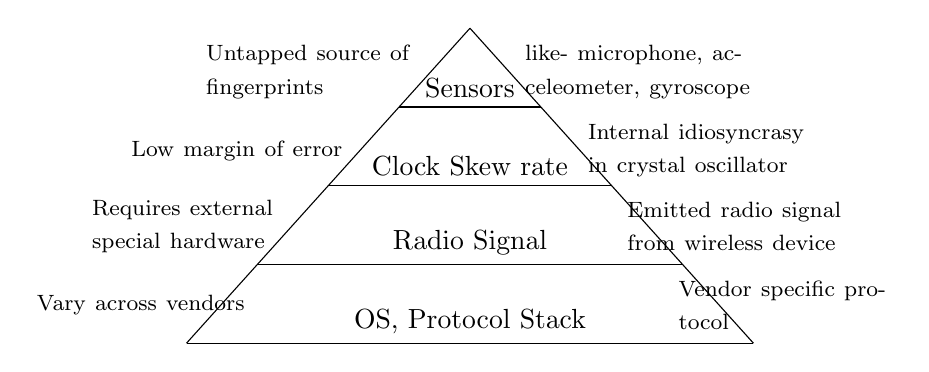
\begin{tikzpicture}[scale=1]

		\def \h {4};
		\def \f {0.9};

		\foreach \y in  {0,1,2,3} {
		    \def \w { \h*\f-\y*\f };
		    \def \v { \y*\f-\h*\f };
		    \draw (\v,\y) -- (\w,\y);
		}

		\draw (-\h*\f,0)  -- (0,\h);
		\draw (\h*\f,0)  -- (0,\h);
		\node (os) at (0,0) [above] {OS, Protocol Stack};
		\node (rf) at (0,1) [above] {Radio Signal};
		\node (cs) at (0,2) [above] {Clock Skew rate};
		\node (se) at (0,3) [above] {Sensors};


		\node [left of=os, xshift=-3cm, yshift=0.2cm, text width=3cm] {\footnotesize{Vary across vendors}};
		\node [left of=rf, xshift=-2.4cm, yshift=0.2cm, text width=2.8cm] {\footnotesize{Requires external special hardware}};
		\node [left of=cs, xshift=-1.8cm, yshift=0.2cm, text width=3cm] {\footnotesize{Low margin of error}};
		\node [left of=se, xshift=-1cm, yshift=0.2cm, text width=2.7cm] {\footnotesize{Untapped source of fingerprints}};

		\node [right of=os, xshift=3cm, yshift=0.2cm, text width=2.7cm] {\footnotesize{Vendor specific protocol}};
		\node [right of=rf, xshift=2.5cm, yshift=0.2cm, text width=3cm] {\footnotesize{Emitted radio signal from wireless device}};
		\node [right of=cs, xshift=2cm, yshift=0.2cm, text width=3cm] {\footnotesize{Internal idiosyncrasy in crystal oscillator}};
		\node [right of=se, xshift=1.2cm, yshift=0.2cm, text width=3cm] {\footnotesize{like- microphone, acceleometer, gyroscope}};
	\end{tikzpicture}
	\caption{\label{fig:pyramid} The pyramid of features in a mobile device that can be used for fingerprinting.\cite[]{sensor:acoustic}}
\end{figure}

As seen above in~\figureref{fig:pyramid} are sensors an untapped source of fingerprints in mobile devices and example of sensors are microphone, accelerometer, barometer, speakers and gyroscope. The sensors investigated in this work is the accelerometer-, gyroscope-, magnetometer- and camera- sensors. All of them are common sensors in most of the mobile devices used today.


\section{Accelerometer\index{accelerometer}}\label{sec:accelerometer}
The accelerometer is the sensor that detect movement on a mobile device, like when you changing orientation on your device. Acceleration is measured by sensing how much pressure the device has in terms of force. The type of accelerometer sensor found in a mobile device is a micro-electromechanical systems known as MEMS sensor. \cite[]{sensors:fusion}
\subsection{Fingerprinting feature / Bias}
Measure the characteristics from the accelerometer is done by taking the long term average of the output when the accelerometer is in rest. That is the biggest error source in the accelerometer and it grows quadratically over time, but when the accelerometer is in rest the error $\epsilon$ can be calculated as a function of time $t$;
\begin{equation} \label{eq:AccBias}
s(t)=\epsilon * \frac{t^2}{2} 
\end{equation}
\cite[]{sensor:inertialNav}\cite[]{sensors:fusion}


\section{Gyroscope\index{gyroscope}}\label{sec:gyroscope}
The gyroscope is sensing how the device is moving in terms of angles, for maintaining or measure the orientation. This is originally  a mechanical system based on the principle of conservation of angular momentum. The most popular Gyroscope for devices today is a MEMS that is using silicon micro-mechanical techniques. Coriolis effect is measured with vibrating elements in the MEMS gyroscope. Coriolis effect is a change of moving objects direction when looking at it from a rotating reference system. The difference from the accelerometer is that the gyroscope measures relative to the device body rather than relative to earth. The equations of Coriolis force;  
$$\boldsymbol{ F}_C = -2 \, m \, (\omega *  v)$$
Where $m$ is the mass of the particle, $\omega$ the angular velocity and $v$ the velocity of the particle in the rotating system. 
\cite[]{sensor:inertialNav}
\subsection{Fingerprinting feature / Bias}
The gyroscope has some error characteristics like constant bias, white noise, bias instability, calibration error and temperature effects. One of these error characteristics that can be tested by reading the output from a gyroscope in rest is the \textit{constant bias}\index{constant bias}. That is bias of the gyroscope output when not having any rotation on it. This constant error $\epsilon$ of the bias over time $t$ leads to an angular error that grows linear; 
\begin{equation} \label{eq:gyroBias}
\theta (t)= \epsilon * t
\end{equation}
If take the long term average output from the gyro in rest, the constant error of a rate gyro can be estimated.\cite[]{sensors:fusion}


\section{Magnetometer\index{magnetometer}}
The magnetometer measures the magnetic field and was originally used for navigation and tracking. When it is used as a compass the Earth's magnetic field is measured. The type of sensor found in mobile devices is like accelerometer and gyroscope a MEMS sensor. They are known as e-compasses gaussmeters that is measuring of magnetic fields larger than 1 nT.
~\cite[]{sensor:magn}

\subsection{Fingerprinting feature / Bias}
\textit{Note that normally bias in a magnetometer is called \textbf{offset} but for uniformity reason of this report it will be referenced to \textbf{bias}.}\\
When try to measure the magnetic field of Earth with a magnetometer it also gets affected by other magnetic fields. The two main error sources from measurements of magnetometer are magnetic contamination in the sensor, called Soft and Hard-Iron distortion. \\
The hard iron distortion is caused by metals and magnets around the magnetometer. This field is constant even if the device moves, thus it is additive to the earths magnetic field. This distortion can be caused of e.g. the device speaker mounted near the magnetometer. \\
If there are magnetic fields in the surrounding environment of the device they will cause soft iron disorder. This error is smaller than the hard iron distortion. Any metal around the device can cause this error, such a car passing by.
There are also a third bias that can effect the magnetometer and is as the hard iron distortion additive. This bias is the errors in the magnetometer itself such that all hardware has. But the result of this bias is similar to the soft iron distortion.  \\
The good thing with magnetometer bias is that it is constant over time, thus once it is calculated it stays the same. \\
\\
If the device is rotated one turn (360\degree)around its own z-axes (see~\figureref{fig:device-axes}) and plot x with respect to y there will be a circle. In a world without bias this circle will look like:
\begin{figure}[H]
\begin{tabular}{p{0.23\textwidth} p{0.23\textwidth} p{0.23\textwidth} p{0.23\textwidth}}
        \vspace{0pt} \begin{tikzpicture}[line cap=round,line join=round,>=triangle 45,x=1.0cm,y=1.0cm]
\draw[->,color=black] (-1.5,0.) -- (1.5,0.);
\foreach \x in {-1.4,-1.2,-1.,-0.8,-0.6,-0.4,-0.2,0.2,0.4,0.6,0.8,1.,1.2,1.4}
\draw[shift={(\x,0)},color=black] (0pt,-2pt);
\draw[color=black] (1.3548383992423667,0.012646598999199708) node [anchor=south west] {X};
\draw[->,color=black] (0.,-1.5) -- (0.,1.5);
\foreach \y in {-1.4,-1.2,-1.,-0.8,-0.6,-0.4,-0.2,0.2,0.4,0.6,0.8,1.,1.2,1.4}
\draw[shift={(0,\y)},color=black] (-2pt,0pt);
\draw[color=black] (0.015808248748999637,1.4306334471160802) node [anchor=west] {Y};
\clip(-1.5,-1.5) rectangle (1.5,1.5);
\draw(0.,0.) circle (1.cm);
\begin{scriptsize}
\draw [color=xdxdff] (0.,0.)-- ++(-2.0pt,-2.0pt) -- ++(4.0pt,4.0pt) ++(-4.0pt,0) -- ++(4.0pt,-4.0pt);
\draw [fill=qqqqff] (0.,1.) circle (1.5pt);
\draw[color=qqqqff] (-0.15,1.1) node {0\textrm{\degre}};
\end{scriptsize}
\end{tikzpicture}
 & 
        \vspace{0pt} \begin{tikzpicture}[line cap=round,line join=round,>=triangle 45,x=1.0cm,y=1.0cm]
\draw[->,color=black] (-1.5,0.) -- (1.5,0.);
\foreach \x in {-1.4,-1.2,-1.,-0.8,-0.6,-0.4,-0.2,0.2,0.4,0.6,0.8,1.,1.2,1.4}
\draw[shift={(\x,0)},color=black] (0pt,-2pt);
\draw[color=black] (1.3548383992423672,0.012646598999199708) node [anchor=south west] {X};
\draw[->,color=black] (0.,-1.5) -- (0.,1.5);
\foreach \y in {-1.4,-1.2,-1.,-0.8,-0.6,-0.4,-0.2,0.2,0.4,0.6,0.8,1.,1.2,1.4}
\draw[shift={(0,\y)},color=black] (-2pt,0pt);
\draw[color=black] (0.015808248748999637,1.4306334471160802) node [anchor=west] {Y};
\clip(-1.5,-1.5) rectangle (1.5,1.5);
\draw(-0.2,-0.2) circle (1.003958800671448cm);
\begin{scriptsize}
\draw [fill=qqqqff] (-0.18558461983368865,0.8038553034478191) circle (1.5pt);
\draw[color=qqqqff] (-0.16,1) node {0\textrm{\degre}};
\draw [color=xdxdff] (-0.2,-0.2)-- ++(-2.0pt,-2.0pt) -- ++(4.0pt,4.0pt) ++(-4.0pt,0) -- ++(4.0pt,-4.0pt);
\end{scriptsize}
\end{tikzpicture} & 
        \vspace{0pt} \begin{tikzpicture}[line cap=round,line join=round,>=triangle 45,x=1.0cm,y=1.0cm]
\draw[->,color=black] (-1.5002742877331638,0.) -- (1.5002742877331638,0.);
\foreach \x in {-1.4,-1.2,-1.,-0.8,-0.6,-0.4,-0.2,0.2,0.4,0.6,0.8,1.,1.2,1.4}
\draw[shift={(\x,0)},color=black] (0pt,-2pt);
\draw[color=black] (1.3548383992423672,0.012646598999199708) node [anchor=south west] {X};
\draw[->,color=black] (0.,-1.500215870948452) -- (0.,1.5001897416116785);
\foreach \y in {-1.4,-1.2,-1.,-0.8,-0.6,-0.4,-0.2,0.2,0.4,0.6,0.8,1.,1.2,1.4}
\draw[shift={(0,\y)},color=black] (-2pt,0pt);
\draw[color=black] (0.015808248748999637,1.4306334471160802) node [anchor=west] {Y};
\clip(-1.5002742877331638,-1.500215870948452) rectangle (1.5002742877331638,1.5001897416116785);
\draw [rotate around={-36.86989764584405:(0.,-0.15)}] (0.,-0.15) ellipse (1.1608455676650522cm and 0.8860374890305703cm);
\begin{scriptsize}
\draw [color=xdxdff] (0.04907705257499707,-0.12173658003568395)-- ++(-2.0pt,-2.0pt) -- ++(4.0pt,4.0pt) ++(-4.0pt,0) -- ++(4.0pt,-4.0pt);
\draw [fill=qqqqff] (-0.8962562226151813,0.5864729639194997) circle (1.5pt);
\draw[color=qqqqff] (-1.1,0.75) node {0\textrm{\degre}};
\end{scriptsize}
\end{tikzpicture} & 
        \vspace{0pt} \begin{tikzpicture}[line cap=round,line join=round,>=triangle 45,x=1.0cm,y=1.0cm]
\draw[->,color=black] (-1.500130470417328,0.) -- (1.5002743955178048,0.);
\foreach \x in {-1.4,-1.2,-1.,-0.8,-0.6,-0.4,-0.2,0.2,0.4,0.6,0.8,1.,1.2,1.4}
\draw[shift={(\x,0)},color=black] (0pt,-2pt);
\draw[color=black] (1.3548385432174719,0.012646598999199708) node [anchor=south west] {X};
\draw[->,color=black] (0.,-1.500215870948452) -- (0.,1.5001897416116785);
\foreach \y in {-1.4,-1.2,-1.,-0.8,-0.6,-0.4,-0.2,0.2,0.4,0.6,0.8,1.,1.2,1.4}
\draw[shift={(0,\y)},color=black]  (-2pt,0pt);
\draw[color=black] (0.015808244815253596,1.4306334471160802) node [anchor=west] {Y};
\clip(-1.500130470417328,-1.500215870948452) rectangle (1.5002743955178048,1.5001897416116785);
\draw [rotate around={0.059845574260994405:(4.8164851529053886E-4,7.838801032565946E-4)}] (4.8164851529053886E-4,7.838801032565946E-4) ellipse (1.2496624710485813cm and 0.9992161789727994cm);
\begin{scriptsize}
\draw [color=xdxdff] (0.,0.)-- ++(-2.0pt,-2.0pt) -- ++(4.0pt,4.0pt) ++(-4.0pt,0) -- ++(4.0pt,-4.0pt);
\draw [fill=qqqqff] (0.,1.) circle (1.5pt);
\draw[color=qqqqff] (-0.15,1.1) node {0\textrm{\degre}};
\end{scriptsize}
\end{tikzpicture} \\
        \vspace{0pt} Ideal & Hard Iron distortion & Soft Iron distortion & Gain mismatch \\
\end{tabular}
\caption{Example of different magnetometer readings when affected by bias.}\label{fig:magnCircle}
\end{figure}
\cite[]{liu:magnAcc}

\subsection{Magnetometer calibration}
To do a magnetometer calibration the device is turned 360\degree around the z-axis (~\figureref{fig:device-axes}), with the device on a flat surface. This makes x and y-axis the surface and z-axis pointing (UP/DOWN?). To calculate the offset $O_{x,y,z}$ the average of min and max-value from each axis is calculated (the center of the circle) from the magnetic field $B_{x,y,z}$, like:
\begin{subequations}
\begin{align}
  O_x = \frac{max(B_x) + min(B_x)}{2} \\
  O_y = \frac{max(B_y) + min(B_y)}{2} \\
  O_z = \frac{max(B_z) + min(B_z)}{2}
\end{align} 
And the hard iron compensated result $m_{x,y,z}^h$:
\begin{align}
  m_x^h = B_x - O_x \\
  m_y^h = B_y - O_y \\
  m_z^h = B_z - O_z
\end{align}
\end{subequations}
The soft iron is sometimes compensated for in the equations above and sometimes additional compensation has to be done. Since soft iron offset is place specific it will not be considered in the thesis since a fingerprint of a device is not convenient if you have to be at the exact same spot every time the device tries to authenticate.
\cite[]{liu:magnAcc}


\section{Camera}\label{sec:char:camera}\index{camera fingerprinting}\index{camera}
\textit{Note that normally bias in a camera sensor is called \textbf{noise} but for uniformity reason of this report it will be referenced to \textbf{bias}.}\\
\\
The digital camera of a mobile device also includes sensors and other hardware that can be used as fingerprinting characteristics. The basic is that light travels trough a lens and hits a imaging sensor which contains pixels that has a filter array in front. The filter is for gives each pixel a detected color. The pixels is then put together again to a resulting signal which is send to some final post processing (color correction, white balance, etc.) steps before the image is written to the memory card. In this process there are different kind of bias that effects the image;
\begin{itemize}
	\item[] \textit{\index{shot noise}Shot noise -} the amount of photons hitting the sensor and each pixel varies a random amount
	\item[] \textit{\index{fixed pattern noise}Fixed pattern noise - }there is a small electric current that leaks from photo-diodes in each pixel, caused by dark current
	\item[] \textit{\index{photo-response non-uniformity noise}\index{PRNU}Photo-response non-uniformity noise (PRNU) -} is a bias that is not affected by temperature or humidity. When manufacturing sensors the silicon gets imperfection which causes that pixels aren't equally sensitive to light. This is the main source of pattern bias and makes it really unlikely for two cameras to have the same pattern.
\end{itemize}
The three types of bias can be described as a mathematical model for getting the output of the sensor $y_{ij}$:
$$y_{ij}=f_{ij}(x_{ij}+\eta_{ij})+c_{ij}+\epsilon_{ij}$$
where $f_{ij}$ is a multiple factor close to one that captures PRNU, $x_{ij}$ is the number of photons hitting the sensor, $\eta_{ij}$ the shot noise, $c_{ij}$ the dark current and $\epsilon_{ij}$ the additive random bias. The key for a unique fingerprint of the camera (in the mobile device) is to finding $f$.
\cite[]{sensor:camera:DCIdent}


\section{Measurements of sensors on mobile devices}\label{sec:charMeasureSensor}
Measurements of sensors from mobile devices can be gather in different ways. In the work of this thesis two approaches is used, a browser application and an Android application. The camera is an exception where pictures provides the sensor characteristics.
\begin{figure}[H]
	\centering
    \includegraphics[scale=0.2]{img/device-axes}
    \caption{The coordinate system used for both Android and JavaScript\cite[]{sensor:W3C}}
  \label{fig:device-axes}
\end{figure}

\subsection{Android}\label{subsec:Android}\index{Android}
Android sensor framework provides raw data with high precision from sensor that are built in the device such as different motions sensors (including accelerometer and gyroscope), environmental sensors and position sensors (e.g. magnetometer). \cite[]{android:sensor}
Android sensor framework classes that is used for gather sensor data is; 
\begin{itemize}
	\item[] \texttt{SensorManager}, a manager used to access the sensor of the device. 
	\item[] \texttt{Sensor}, representing a sensor
	\item[] \texttt{SensorEvent}, an event from a Sensor such data from the sensor, time-stamp or accuracy
	\item[] \texttt{SensorEventListener}, gets a SensorEvent when a sensor or accuracy has changed 
\end{itemize}
In Android you can't just read from the sensor whenever you need, instead the SensorEventListener has a function that is triggered every time the sensor is changed. You can however set how fast the delay from the sensor should be. The function provides the output of the sensor with a time-stamp of when (in nanoseconds) the change occured. The template code for this function:
\lstinputlisting{code/android-sensor.java}\label{code:androidSensor}
\cite[]{android:sensorEvent} 




\subsubsection{Accelerometer in Android}\label{subsec:accAndroid}
\texttt{TYPE\_ACCELEROMETER} is the hardware measurements that measures the force of acceleration including the force of gravity with the SI unit $m/s^2$. Android also provide \texttt{TYPE\_LINEAR\_ACCELERATION} that is without gravity but that is a combined hardware and software sensor, thus this tests uses  \texttt{TYPE\_ACCELEROMETER} that provides almost raw data. There have been some bias removal from the sensor such bias from different temperature. \\
To get the acceleration applied to the device ($a_d$) the measurements of the force ($F_s$) applied the sensor is calculated from Newtons second law using the mass ($m$) of the device :
$$a_d=-\sum F_s / m $$ 
These measurements from the \texttt{SensorEvent} is in the x-,y- and z-axes like in~\figureref{fig:device-axes} and collected from event like x=a, y=b and z=c in~\ref{code:androidSensor}. \cite[]{android:sensorEvent}


\subsubsection{Gyroscope in Android}\label{subsec:gyroAndroid}
The data from the gyroscope sensor is collected from the \texttt{TYPE\_GYROSCOPE} that measures the rotation in rad/s around the x-, y- and z-axis of~\figureref{fig:device-axes}. The direction of the rotation is positive counter-clockwise if looking from a positive location of the axes. The values from the measurements when the gyroscope is changed is given like rotation in x=a, y=b and z=c in~\ref{code:androidSensor}. Additional output is \texttt{values[3], values[4]} and \texttt{values[5]} that is the estimated drift arounf the axis in also in rad/s.\\
Android also provide a \texttt{TYPE\_GYROSCOPE\_UNCALIBRATED} that is the same as \texttt{TYPE\_GYROSCOPE} except that no drift has been compensated for. There is still factory calibration and temperature compensation applied. \cite[]{android:sensorEvent} This makes it possible to calculate the linear sensor bias (equation~\ref{eq:gyroBias}] without Androids own bias compensation that is not known what it is.



\subsubsection{Magnetometer in Android}\label{subsec:magnAndroid}
Measures the magnetic field in x-, y- and z-axis in micro-Tesla ($\mu T$), as for the other sensors is that output for \texttt{values[0], values[1]} and \texttt{values[2]} (see code~\ref{code:androidSensor}). Android also provides a uncalibrated version that not has any calibration for the hard iron calibration. The uncalibrated type in Android is \texttt{TYPE\_MAGNETIC\_FIELD\_UNCALIBRATED} and as for the gyrocope it also comes with an bias estimation in x, y and z-axis for event-values \texttt{values[3], values[4]} and \texttt{values[5]}. 

\subsubsection{Fingerprinting: Sensor fusion in Android}
\url{http://www.codeproject.com/Articles/729759/Android-Sensor-Fusion-Tutorial}

\subsection{JavaScript}\label{subsec:js}\index{JavaScript}
JavaScript has since the use of smart-phones adapted a lot of new features, which makes it possible to access a lot of features in the devices. To access the gyroscope and accelerometer-data no permission from the user is needed, thus the user do not have to know that the sensors are measured.


\subsubsection{Accelerometer in JavaScript}\label{subsec:accJS}
To get measurements from the accelerometer an event listener called \texttt{devicemotion} is added. The output from measurements is the acceleration force in $m/s^2$ according to x-, y- and z-axes as in~\figureref{fig:device-axes}. \\
\\
In JavaScript there are two types of acceleration, \texttt{accelerationIncludingGravity} and \texttt{acceleration}.\texttt{accelerationIncludingGravity} is acceleration made by the device. In context to \texttt{acceleration} not depending on influence of gravity only by the acceleration made on the device. Since the accelerometer in the device measures with gravity I assume that that is the most raw data you can get of the two. There is no documentation on this made, thus that makes this some kind of a guess.\\
\\
The JavaScript for measurements of the accelerometer:
\lstinputlisting{code/acc-listener.js}
\cite[]{sensor:W3C}


\subsubsection{Gyroscope in JavaScript}\label{subsec:gyroJS}
A listener is implemented in the same way as for the accelerometer, this listener is called  \texttt{deviceorientation}. The output from this listener is made in degrees of rotation angle. JavaScript has named this rotations as the~\figureref{fig:device-rot} below.
\begin{figure}[H]
  \hspace{-1cm}
  \centering
  \begin{minipage}[c]{.23\textwidth}
    \centering
    \includegraphics[scale=0.2]{img/device-alpha}
  \end{minipage}
  \hspace{1cm}
  \begin{minipage}[c]{.23\textwidth}
    \centering
    \includegraphics[scale=0.2]{img/device-beta}
  \end{minipage}
  \hspace{1cm}
  \begin{minipage}[c]{.23\textwidth}
    \centering
    \includegraphics[scale=0.2]{img/device-gamma}
    \hspace{1cm}
  \end{minipage}
  \caption{The device rotation axes for the JavaScript \texttt{DeviceOrientation}}
  \label{fig:device-rot}
\end{figure}
Alpha is measured in the range of 0\degree to 360\degree around the z-axis, beta in in the range of -180\degree to 180\degree around x-axis and gamma in the range of -90\degree to 90\degree around y-axis.\\
\\
The JavaScript for measurements of the gyroscope:
\lstinputlisting{code/gyro-listener.js}
\cite[]{sensor:W3C}

\chapter{METHOD OF MEASUREMENTS}\label{cha:measurements}
In this chapter the methods used for testing the mobile devices for different characteristics is described in~\chapterref{cha:character}. Different test where performed to get sensor data to analyze for bias and characteristics. \\
\\
Overview of the tests performed:
\begin{itemize}
  \item[] \textbf{Measurement I - Motion:} Collected accelerometer and gyroscope data by using a JavaScript web-page. The purpose to find out which of \texttt{accelerationIncludingGravity} and \texttt{acceleration} is better in purpose of extract unique device characteristics.
  \item[] \textbf{Measurement II - Motion:} Collected accelerometer and gyroscope data by using a JavaScript web-page. The purpose to find unique device characteristics from the sensors. 
  \item[] \textbf{Measurement II - Camera:} Collect one video from each device and extract pictures frames from the video. Calculate and compare the PRNU of the extracted pictures. (The videos where collected in the same process as test II above).
  \item[] \textbf{Measurement III - Camera:} Collected ten pictures instead of video from the device. 
\end{itemize}

\section{Measurements of sensors on mobile devices}\label{sec:charMeasureSensor}
Measurements of sensors from mobile devices can be gather in different ways. In the work of this thesis two approaches is used, a browser application and an Android application. The camera is an exception where pictures provides the sensor characteristics.
\begin{figure}[H]
	\centering
    \includegraphics[scale=0.2]{img/device-axes}
    \caption{The coordinate system used for both Android and JavaScript\cite[]{sensor:W3C}}
  \label{fig:device-axes}
\end{figure}

\subsection{Android}\label{subsec:Android}\index{Android}
\textbf{==== OBS: Är detta mer relevant att ha i demo-delen?} \\
Android sensor framework provides raw data with high precision from sensor that are built in the device such as different motions sensors (including accelerometer and gyroscope), environmental sensors and position sensors (e.g. magnetometer). \cite[]{android:sensor}
Android sensor framework classes that is used for gather sensor data is; 
\begin{itemize}
	\item[] \texttt{SensorManager}, a manager used to access the sensor of the device. 
	\item[] \texttt{Sensor}, representing a sensor
	\item[] \texttt{SensorEvent}, an event from a Sensor such data from the sensor, time-stamp or accuracy
	\item[] \texttt{SensorEventListener}, gets a SensorEvent when a sensor or accuracy has changed 
\end{itemize}
In Android you can't just read from the sensor whenever you need, instead the SensorEventListener has a function that is triggered every time the sensor is changed. You can however set how fast the delay from the sensor should be. The function provides the output of the sensor with a time-stamp of when (in nanoseconds) the change occurred. The template code for this function:
\lstinputlisting[caption={Java code for Android sensor},label={code:androidSensor},language=Java]{code/android-sensor.java}
\cite[]{android:sensorEvent} 




\subsubsection{Accelerometer in Android}\label{subsec:accAndroid}
\texttt{TYPE\_ACCELEROMETER} is the hardware measurements that measures the force of acceleration including the force of gravity with the SI unit $m/s^2$. Android also provide \texttt{TYPE\_LINEAR\_ACCELERATION} that is without gravity but that is a combined hardware and software sensor, thus this tests uses  \texttt{TYPE\_ACCELEROMETER} were the measurements only comes from hardware. There have been some bias removal from the sensor such bias from different temperature. \\
To get the acceleration applied to the device ($a_d$) the measurements of the force ($F_s$) applied the sensor is calculated from Newtons second law using the mass ($m$) of the device :
$$a_d=-\sum F_s / m $$ 
These measurements from the \texttt{SensorEvent} is in the x-,y- and z-axes like in~\figureref{fig:device-axes} and collected from event like x=a, y=b and z=c in~\coderef{code:androidSensor}. \cite[]{android:sensorEvent}


\subsubsection{Gyroscope in Android}\label{subsec:gyroAndroid}
The data from the gyroscope sensor is collected from the \texttt{TYPE\_GYROSCOPE} that measures the rotation in rad/s around the x-, y- and z-axis of~\figureref{fig:device-axes}. The direction of the rotation is positive counter-clockwise if looking from a positive location of the axes. The values from the measurements when the gyroscope is changed is given like rotation in x=a, y=b and z=c in ~\coderef{code:androidSensor}. Additional output is \texttt{values[3], values[4]} and \texttt{values[5]} that is the estimated drift arounf the axis in also in rad/s.\\
Android also provide a \texttt{TYPE\_GYROSCOPE\_UNCALIBRATED} that is the same as \texttt{TYPE\_GYROSCOPE} except that no drift has been compensated for. There is still factory calibration and temperature compensation applied. \cite[]{android:sensorEvent} This makes it possible to calculate the linear sensor bias (equation~\ref{eq:gyroBias}] without Androids own bias compensation that is not known what it is.



\subsubsection{Magnetometer in Android}\label{subsec:magnAndroid}
Measures the magnetic field in x-, y- and z-axis in micro-Tesla ($\mu T$), as for the other sensors is that output for \texttt{values[0], values[1]} and \texttt{values[2]} (~\coderef{code:androidSensor}). Android also provides a uncalibrated version that not has any calibration for the hard iron calibration. The uncalibrated type in Android is \texttt{TYPE\_MAGNETIC\_FIELD\_UNCALIBRATED} and as for the gyrocope it also comes with an bias estimation in x, y and z-axis for event-values \texttt{values[3], values[4]} and \texttt{values[5]}. 


\subsection{JavaScript}\label{subsec:js}\index{JavaScript}
JavaScript has since the use of mobile devices adapted a lot of new features, which makes it possible to access a lot of hardware features in the devices. No permission is needed to access the gyroscope and accelerometer-data, thus the user do not have to know that the sensors are measured.


\subsubsection{Accelerometer in JavaScript}\label{subsec:accJS}
To get measurements from the accelerometer an event listener called \texttt{devicemotion} is added. The output from measurements is the acceleration force in $m/s^2$ according to x-, y- and z-axes as in~\figureref{fig:device-axes}. \\
\\
In JavaScript there are two types of acceleration, \texttt{accelerationIncludingGravity} and \texttt{acceleration}. The \texttt{accelerationIncludingGravity} is acceleration made by the device. In context to \texttt{acceleration} not depending on influence of gravity only by the acceleration made on the device. What this actually means is that if a device lies still with the screen facing upwards the \texttt{acceleration} output will be zero in x, y and z-axes but the \texttt{accelerationIncludingGravity} will be zero along x and y-axes, the z-axis will be equal to G. If you put the device in free fall with the screen facing upwards the acceleration is zero with \texttt{accelerationIncludingGravity} and x=0,y=0 and z=-G for the \texttt{acceleration}. \cite{sensor:W3Cspec} \\
The rotation rate of the device is also available from the \texttt{devicemotion}, that is the acceleration ($m/s^2$) around the axes as seen in \figureref{fig:device-rot}. \\
\\
The JavaScript for measurements of the accelerometer:
\lstinputlisting{code/acc-listener.js}
\cite[]{sensor:W3C}


\subsubsection{Gyroscope in JavaScript}\label{subsec:gyroJS}
A listener is implemented in the same way as for the accelerometer, this listener is called  \texttt{deviceorientation}. The output from this listener is made in degrees of rotation angle. JavaScript has named this rotations as the~\figureref{fig:device-rot} below.
\begin{figure}[H]
  \hspace{-1cm}
  \centering
  \begin{minipage}[c]{.23\textwidth}
    \centering
    \includegraphics[scale=0.2]{img/device-alpha}
  \end{minipage}
  \hspace{1cm}
  \begin{minipage}[c]{.23\textwidth}
    \centering
    \includegraphics[scale=0.2]{img/device-beta}
  \end{minipage}
  \hspace{1cm}
  \begin{minipage}[c]{.23\textwidth}
    \centering
    \includegraphics[scale=0.2]{img/device-gamma}
    \hspace{1cm}
  \end{minipage}
  \caption{The device rotation axes for the JavaScript \texttt{DeviceOrientation}}
  \label{fig:device-rot}
\end{figure}
Alpha is measured in the range of 0\degree to 360\degree around the z-axis, beta in in the range of -180\degree to 180\degree around x-axis and gamma in the range of -90\degree to 90\degree around y-axis.\\
\\
The JavaScript for measurements of the gyroscope:
\lstinputlisting{code/gyro-listener.js}
\cite[]{sensor:W3C}

\section{Measurement I - Motion}\label{sec:measurementI}
The first measurement had the purpose to test the accelerometer with and without the impact of gravity. This with the purpose to see if any of them where a better choice in terms of characteristics uniqueness in the devices.\\
The data were collected by developing a JavaScript web-page that used the listeners described in~\sectionref{subsec:accJS}. The test where completely diverse in sense of device platform and only required a browser installed and Internet connection. 
This only require that the measured device has Internet connection and a browser installed, no additional installations and completely cross-platform.\\
\\
The measurements required that the device where still on a flat surface, then started by pressed a button. It gathered 1000 samples of accelerometer data that where saved as a CSV-file for further analyzing. It also collected gyroscope data as well for possible future analyzing purposes. The screen-shots below shows the web-page while measuring and the right one when finished and ready to send. 
\begin{figure}[H]
  \hspace{-2cm}
  \centering
  \begin{minipage}[c]{.23\textwidth}
    \centering
    \includegraphics[scale=0.1]{img/Nexus-rec}
  \end{minipage}
  \hspace{2cm}
  \begin{minipage}[c]{.23\textwidth}
    \centering
    \includegraphics[scale=0.1]{img/Nexus-submit}
  \end{minipage}
  \caption{Screen-shots of web-page during accelerometer measurements in test I}
  \label{fig:gyrotion}
\end{figure}

\section{Measurement II - Motion}\label{sec:measurementII}
The second measurements where also performed from a web-page using JavaScript to collect gyroscope and accelerometer data and a file-upload to collect measurements from the camera of the device. As of the result in last test there where a few changes made to improve the accuracy of the measurements and to collect sensor samples from the gyroscope and camera:
\begin{enumerate}
  \item Adding time-stamp to every recording sample to know exactly recording frequency to enable further analyzing.
  \item Time based recording on 30 seconds instead of taking 1000 samples as in the first test (~\sectionref{sec:measurementI}).
  \item It's also sampling at a lower rate of at least 10 ms instead of as fast as it could before to reduce the effect of other processes that may are in use on the device.
  \item Accelerometer listener used is only \texttt{accelerationIncludingGravity}, due to results described in ~\sectionref{res:testI}.
  \item Added a listener for the gyroscope, ~\sectionref{subsec:gyroJS}.
  \item Collecting camera sensor by a five seconds black video, ~\sectionref{sec:measurement:camera}.
\end{enumerate}

\begin{figure}[H]
  \hspace{-2cm}
  \centering
  \begin{minipage}[c]{.23\textwidth}
    \centering
    \includegraphics[scale=0.15]{img/sensorrec-nexus-2-notRec}
  \end{minipage}
  \hspace{2cm}
  \begin{minipage}[c]{.23\textwidth}
    \centering
    \includegraphics[scale=0.15]{img/sensorrec-nexus-1-rec}
  \end{minipage}
  \caption{Motion sensor measurements II on a Google Nexus 7}
  \label{fig:sensorrec}
\end{figure}

\section{Camera measurements}\label{sec:measurement:camera}
As most of the camera fingerprinting articles (REFERENSER!!) has mostly been in forensic purposes and not focusing on the measurability or integrity of the pictures. That is why some limitations has been made in these measurements. The black motive is used due to integrity, thus no information that could reveal the environment surrounding the camera is sent. Because of measurability (~\sectionref{auth:bio:character})) limited number of pictures that can be taken in a enrollment phase of a device fingerprinting authentication system.\\

To measure the camera two measurements where gathered in both cases where the device on a flat surface which makes the camera result black. Both of this measurements is analyzed by the PRNU-method used by~\cite{sensor:camera:DCIdent} described in~\sectionref{sec:ResCam}.
\begin{enumerate}
  \item \textbf{Black video:} The recommended number of pictures for camera fingerprinting is 50 ~\cite[]{sensor:camera:DCIdent}. But that is not a convenient gathering purposes, thus to ask someone to take 50 black photos and send will not make many answers. Thats why the first test asked for recording a 5 seconds video-recording with the camera towards a flat surface. This video is then shuttered into picture frames, 5 seconds generate 100-200 pictures depending on the recording rate of fps (frames per second).
  \item \textbf{10 black photos:} Simple as taking 10 photos, also with the camera pointing down on a flat surface. Since ~\cite{sensor:camera:DCIdent} where using pictures of diverse motive this aims to investigate if there may be enough with 10 pictures when the motive is the same.
\end{enumerate}

Screen-shots from the camera-page of the second measurements:
\begin{figure}[h!]
  \hspace{-2cm}
  \centering
  \begin{minipage}[c]{.23\textwidth}
    \centering
    \includegraphics[scale=0.15]{img/sensorrec-nexus-3-cam}
  \end{minipage}
  \hspace{2cm}
  \begin{minipage}[c]{.23\textwidth}
    \centering
    \includegraphics[scale=0.15]{img/sensorrec-nexus-4-send}
  \end{minipage}
  \caption{Sensor measurements on a Google Nexus 7}\label{fig:sensorrecCamera}
\end{figure}

For calculating the bias the MATLAB \texttt{medfilt2} is used, which is an 2-D median filtering that outputs the median value of each pixel by its 3-by-3 neighbors. 
\begin{figure}[H]
  \centering
  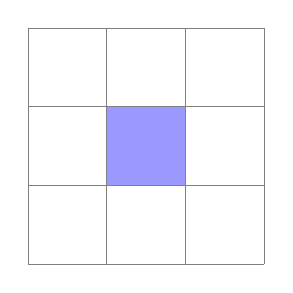
\begin{tikzpicture}[scale=1]
	\draw[step=1cm,gray,very thin] (0,0) grid (3,3);
	\fill[blue!40!white] (1,1) rectangle (2,2);
\end{tikzpicture}
  \caption{\label{fig:medfilt2} the MATLAB \texttt{medfilt2} outputs the median of each pixel by it's 3-by-3 neighbors}
\end{figure}
From the \texttt{medfilt2} is a picture gained without noise which is then subtracted from the original to get the noise. This technique works best if there are no features on the pictures such auto-fix, black and white etc. The more images used for the average value the better noise is, thus the amount random noise is less and the fixed noise is more. \cite{sensor:camera:DCIdent} recommend a minimum of 50 images. This is then seen as the reference pattern used for correlating the noise from another pictures. This correlation is calculated like:
$$
corr(\boldsymbol{n},\boldsymbol{r}) = 
\frac{(\boldsymbol{n} - \bar{\boldsymbol{n}})(\boldsymbol{r} - \bar{\boldsymbol{r}})}
{\|\boldsymbol{n} - \bar{\boldsymbol{n}}\| \|\boldsymbol{r} - \bar{\boldsymbol{r}}\|}
$$
\chapter{RESULT OF MEASUREMENTS}\label{cha:result}
This chapter covers the results of the measurements described in~\chapterref{cha:measurements}. The first two sections cover the measurements made on the accelerometer and gyroscope sensor. Third section cover the result of the two camera measurements.

\section{Pre-measurements}
To get a hint if accelerometer were a possible fingerprinting candidate some pre-measurements were preformed. This were in the early state of the development of the web-page used in measurements I and II. The measurement preformed on six different iPhones showed in~\figureref{fig:iPhoneScatter} indicates that the accelerometer is a sensor that may be good in fingerprinting purposes.
\begin{figure}[H]
\centering
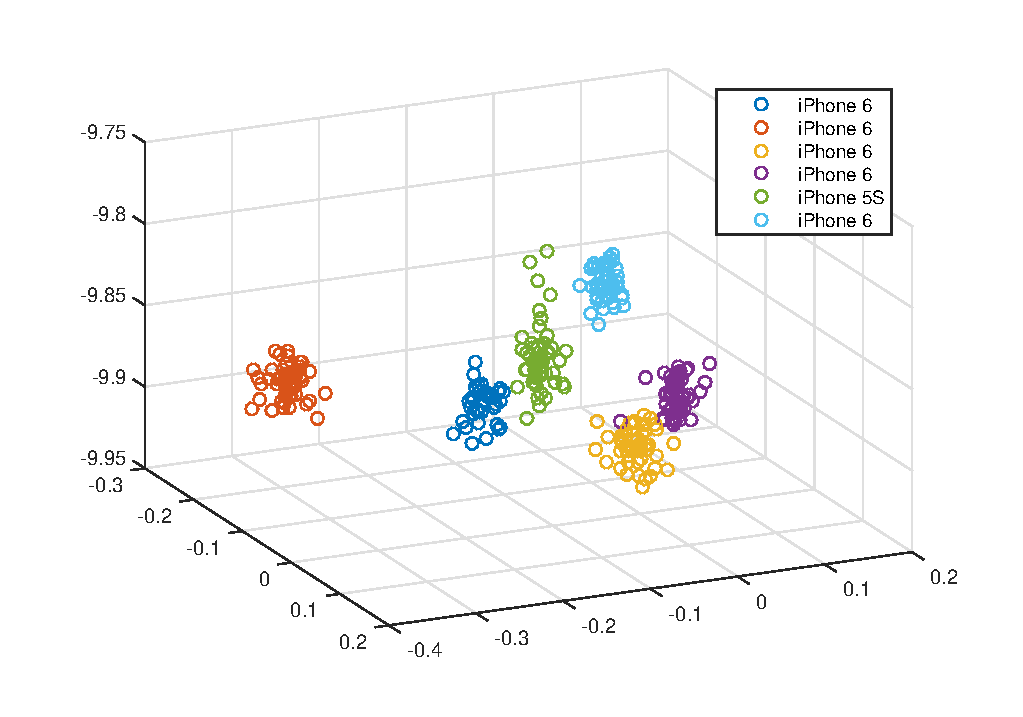
\includegraphics[scale=.6]{img/scatteriPhone}
\caption{Scatter-plot on accelerometer recordings of 6 Apple devices}
\label{fig:iPhoneScatter}
\end{figure}

\section{Result of measurements I  - Motion}\label{res:testI}
The data were gathered as described in~\sectionref{sec:measurementI} from the web-page in \figureref{fig:gyrotion} by spreading the the page. This resulted in over a hundred recordings, which had diversity in platforms, brands and models. Since the web-page where spread mostly to company employees the amount of devices with the same model is high as seen in ~\figureref{fig:measure1-topDevices}.
The purpose of this measurement where to identify if there where differences in terms of bias characteristics between the JavaScript's \texttt{accelerationIncludingGravity} and \texttt{acceleration}. The result of the measurements can be showed by making scatter-plots of the output acceleration of the devices. As shown in the ~\figureref{fig:measure1-topDevices} the \textit{Sony Xperia} devices represents more than a fifth of the total devices in the measurement. 
\begin{figure}[H]
	\centering
	\includegraphics[scale=0.3]{img/measure1-brand}
	\caption{Diversity of device brand sampled in measurements I}
	\label{fig:measure1-brand}
\end{figure}
\begin{figure}[H]
	\centering
	\includegraphics[scale=0.5]{img/measure1-devices}
	\caption{Most common devices models in measurements I}
	\label{fig:measure1-topDevices}
\end{figure}
The result of scatter-plots of measurements of 12 \textit{Sony Xperia} devices with and without gravity in accelerometer readings is shown in~\figureref{fig:scatter-withoutGrav} and~\figureref{fig:scatter-withGrav}.
\begin{figure}[H]
	\centering
	\includegraphics[scale=0.6]{img/res-measure1-scatter-notG}
	\caption{Bias from twelve \textit{Sony Xperia} deives measured with JavaScripts's \texttt{acceleration}}
	\label{fig:scatter-withoutGrav}
\end{figure}
\begin{figure}[H]
	\centering
	\includegraphics[scale=0.6]{img/res-measure1-scatter-inclG}
	\caption{Bias from twelve \textit{Sony Xperia} deives measured with JavaScripts's \texttt{accelerationIncludingGravity}}
	\label{fig:scatter-withGrav}
\end{figure}
As stated in~\cite{acc:kionixerr} the sources of bias in an accelerometer has to be compensated for. The manufacturer of the mobile devices makes some of this compensation before JavaScript gets the data. The results of the figures above indicates that JavaScript also makes compensating to the output of the event \texttt{acceleration}, probably to ease the development of software using the accelerometer, e.g. games. This however is not anything that is public in any specifications such~\cite{sensor:W3Cspec} or~\cite{sensor:accIncludingGravity}. The Android developer page about sensor event \cite{android:sensorEvent} state that they make factory calibration and temperature compensation even on their uncalibrated sensor events of (only magnetometer and gyroscope) that is relativity new feature added in Android 4.3 Jelly Bean (API level 18~\cite{android:API18}) from 2013 but the original once used since Android 1.5 Cupcake (API level 3~\cite{android:API3}) from 2009 makes some more noise compensation and calibration. What kind of compensation and calibration done is not public. 

\section{\textbf{Doing! }Result of measurements II  - Motion}\label{res:testII}
The result here is an analyses of the gyroscope and accelerometer data collected from 60 devices by an improved version of the JavaScript web-page used in measurements I. The changes that were made is described in~\sectionref{sec:measurementII} to improve that analyze data. \\
The diversity of the devices brands in the measurement is shown in the~\figureref{fig:brandII} below.
\begin{figure}[H]
	\centering
	\includegraphics[scale=.4]{img/measure2-brands}
	\caption{Diversity of device brand sampled in measurements II}
	\label{fig:brandII}
\end{figure}

\subsection{Permanence of accelerometer}
When choosing biometric trait one of the factors is permanence described in \sectionref{auth:bio:character}, that is the trait not changing significantly over time. To test this measurement II were performed on a \textit{Sony Xperia Z1 Compact} over a period of 50 days. The choice of device was based on that \textit{Sony Xperia} devices is 30\% of the devices that data is collected from. The same test were also made on a \textit{Google Nexus 7} tablet. The graphs below shows the difference of accelerometer readings over time.
\begin{figure}[H]
	\centering
	\includegraphics[scale=.7]{img/sensrec-nex-z1-acc-x}
	\caption{Accelerometer readings of x-axes on a  \textit{Sony Xperia Z1 Compact} and a \textit{Google Nexus 7} over 50 days}
	\label{fig:x50days}
\end{figure}
\begin{figure}[H]
	\centering
	\includegraphics[scale=.7]{img/sensrec-nex-z1-acc-y}
	\caption{Accelerometer readings of y-axes on a  \textit{Sony Xperia Z1 Compact} and a \textit{Google Nexus 7} over 50 days}
	\label{fig:y50days}
\end{figure}
\begin{figure}[H]
	\centering
	\includegraphics[scale=.7]{img/sensrec-nex-z1-acc-z}
	\caption{Accelerometer readings of z-axes on a  \textit{Sony Xperia Z1 Compact} and a \textit{Google Nexus 7} over 50 days}
	\label{fig:z50days}
\end{figure}
As seen in the figures the \textit{Google Nexus 7} hasn't changed much over the 50 days compared to the \textit{Sony Xperia Z1 Compact} that especially has changed in the y-axis. The reason for the difference of accelerometer change over time may be due to the \textit{Google Nexus 7} has only been in the same place during those 50 days and only used when the tests performed. Unlike Mobile used daily, may be dropped at some time. An additional fact about the measurements is that both devices has changed its OS between measurements 2 and 3. The \textit{Google Nexus 7} from Android KitKat 4.4.4 to Lollipop 5.1.1 and the \textit{Sony Xperia Z1 Compact} from Android KitKat 4.4.4 to CyanogenMod 12.1 ( Android version 5.1.1). \\
To get an perspective on this measurements among more devices the scatter-plot in~\figureref{fig:scatterSony50days} that include the same measurements from \textit{Sony Xperia Z1 Compact} as in~\figureref{fig:x50days},~\figureref{fig:y50days} and~\figureref{fig:z50days}.
\begin{figure}[H]
	\centering
	\includegraphics[scale=.3]{img/senrec-sony_scatter-2}
	\caption{Scatter-plot of accelerometer readings \textit{Sony Xperia}-device, one of them with measurements performed on the same device with 50 days apart.}
	\label{fig:scatterSony50days}
\end{figure} 

\subsection{Features of accelerometer data}\label{sec:featuresAcc}
As in ~\cite{sensor:accelPrint} I used statistical features calculated by the time domain. The features used and calculated as followed:
% === IfTime Gör en egen tabell!!
\begin{figure}[H]
	\centering
	\includegraphics[scale=.35]{img/featureCalc}
	\caption{Calculations of statistical accelerometer features. \\\textit{From~\cite[p.6]{sensor:accelPrint}}}
	\label{fig:accFeatures}
\end{figure}
To compare these features and get a picture of if any of them are good for fingerprinting plots of devices were made. These can be found in~\appendixref{cha:matlabFeaturesPlot}. The chosen devices for the plots is the twelve \textit{Sony Xperia Z}-devices including the \textit{Sony Xperia Z1 Compact} that have measurements over 50 days. It becomes clear in the plots that almost all av the features is not changing over time. The only values that changing is the RMS and that the value would change was known even before because as seen in figure~\ref{fig:scatterSony50days} samples is changing over time, which is directly linked to the RMS.

% ToDo Tabell med värderna från min mobil tillsammans 
% med ngn form av snittdistans mellan punkterna om det går
% Lägga till nexus också!!
\begin{table}[H]
\centering
\begin{tabular}{| p{2cm} | p{1cm} | p{1cm} | p{1cm} | p{1cm} |} 
	\hline
  Feature 	& Day 0 & Day 30 & Day 50 & Median dist. 	\\ \hline
  Mean 		& 0 	& 		& 		& \%		\\ \hline
  Std. dev. & 0 	& 30 	& 50 	& \%	\\ \hline
  Avg. dev 	& 0 	& 30 	& 50 	& \%	\\ \hline
  Skewness 	& 0 	& 30 	& 50 	& \%	\\ \hline
  Kurtosis 	& 0 	& 30 	& 50 	& \%	\\ \hline
  RMS 		& 0 	& 30 	& 50 	& \%	\\ \hline
  Min 		& 0 	& 30 	& 50 	& \%	\\ \hline
  Max 		& 0 	& 30 	& 50 	& \%	\\ \hline
\end{tabular} 
\caption[Table caption text]{Values of features of \textit{Sony Xperia Z1 Compact} over 50 days together with the median distance between points of all measured devices.} \label{table:feature50}
\end{table}

\subsection{Gyroscope}
\textbf{=== OBS!!! ===\\}Lägg till ngn plot och visa hr ostabilt gyroskopet är mellan o säg att inte gå vidare i anays med detta..

\subsection{Simulate authentication of motion sensors in MATLAB}
To test that the features above is way of fingerprinting devices a simulation were performed in MATLAB. The concept is that a fingerprint of all devices is calculated. It contains all the features described in~\sectionref{sec:featuresAcc}. When a new measurement is sent in to the simulation, features are calculated and compared to the once already known devices. The comparing is done by an algorithm that calculates the minimum distance between the features of the input device and the one already known. The distance is then used to decide if there is a match or not. As in biometric system there is a reashhold that decides how far from the values an input can be and sill be a match. This treashhold creates a rate of match error in the system called FRR and FAR (see~\sectionref{sec:bio:measure}). 
%% FAR FRR dör tabell eller ngt

% ========== CAMERA TEST ==========
\section{\textbf{ToUpdate! }Result Camera-measurements}\label{sec:ResCam}
\textbf{ ==== OBS!! ====}\\ Flyttad text som måste skrivas om.\\
\\
For the test of the camera sensor the PRNU value is calculated as an approximation of the algorithm described in section ~\ref{sec:char:camera} and also used by \cite{sensor:camera:DCIdent}. That is the average of multiple pictures used and substantially an approximation of \textit{f}. The first step is to remove the pictures-content which leaves the noise, which is done using a denoising filter. For the test the MATLAB \texttt{medfilt2} is used, which is an 2-D median filtering that outputs the median value of each pixel by its 3-by-3 neighbors. 
\begin{figure}[H]
  \centering
  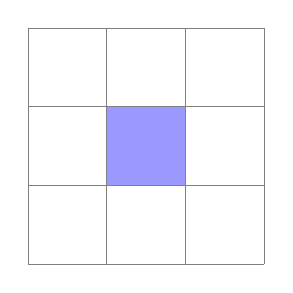
\begin{tikzpicture}[scale=1]
	\draw[step=1cm,gray,very thin] (0,0) grid (3,3);
	\fill[blue!40!white] (1,1) rectangle (2,2);
\end{tikzpicture}
  \caption{\label{fig:medfilt2} the MATLAB \texttt{medfilt2} outputs the median of each pixel by it's 3-by-3 neighbors}
\end{figure}
From the \texttt{medfilt2} we gain a picture without noise which is then subtracted from the original to get the noise. This technique works best if there are no features on the pictures such auto-fix, black and white etc. The more images used for the average value the better noise is, thus the amount random noise is less and the fixed noise is more. \cite{sensor:camera:DCIdent} recommend a minimum of 50 images. This is then seen as the reference pattern used for correlating the noise from another pictures. This correlation is calculated like:
$$
corr(\boldsymbol{n},\boldsymbol{r}) = 
\frac{(\boldsymbol{n} - \bar{\boldsymbol{n}})(\boldsymbol{r} - \bar{\boldsymbol{r}})}
{\|\boldsymbol{n} - \bar{\boldsymbol{n}}\| \|\boldsymbol{r} - \bar{\boldsymbol{r}}\|}
$$
A threshold for acceptance on correlation is found by experimental on images taken with or without the camera. Then there is a balance between FAR and FRR. 
In section ~\ref{sec:measurement:camera} i described two test preformed on the camera sensor of mobile devices.
\subsection{\textbf{ToDo! }Result of camera measurement I}
Since the purpose of this thesis compared to earlier work REFERENSER!! has the purpose of authentication and not forensics, is convenience for the collecting and measurability a factor to take in account. That is why the fist experiment is asked the users to record a 5 seconds video-clip with the device camera facing down on a flat object, like a table. Instead of making the user take 50 pictures or more which takes a lot of more time. This also makes it easier to get better noise since the same scene is used every time. \\
The video is then shuttled into images (100-200 from a 5 seconds video depending on fps on recording camera) that is used for calculating the PRNU. The MATLAB code for this is:\\
\rule{\textwidth}{0.5pt}
  \lstinputlisting{code/video2prnu1.m}
\rule{\textwidth}{0.5pt}

To compare an pictures between all collected PRNU the same calculation to get the noise is done. Then the noise from the reference pictures is compared to all collected PRNU and correlation is calculated like the formula above in MATLAB:\\
\rule{\textwidth}{0.5pt}
  \lstinputlisting{code/corrCamTest1.m}
\rule{\textwidth}{0.5pt}

\subsection{\textbf{ToDo! }Result of camera measurement II}
Since the earlier test leaved out some of the PRNU noise when recorded a video instead of taking a picture the new test consist of 10 images from every device. The recommendation from \cite{sensor:camera:DCIdent} to use at least 50 images is here compensated by again using black images (picture taking with device camera facing down). Since the scene is always the same the noise removal will be better in fewer images. The same code is used as above with the different that the video to image step is removed. The sizes of the images in this case is better since the camera on the mobile devices by default uses higher resolution when taking a picture then when recording. 


\chapter{Demonstration}\label{cha:demo}
Om det blir ngn demo ska den in här.

\section{User Manual}\label{manual}

\section{Choices}
Lite om vilka sensorer jag valde hur jag valzzde dom och varför.
\begin{figure}[!ht]
	\begin{tikzpicture}[node distance=1.6cm]
	\node (start) [justtext] {Start};
	\node (startScreen) [decision, below of=start] {Log in / new device ?};

	\node (vibChallenge) [process, below of=startScreen] {Vibration challenge};
	\node (newDevice) [process, right of=vibChallenge] {New device};

	\node (matchCh) [decision, below of=vibChallenge] {Match?};
	\node (vibCali) [process, below of=newDevice]{Motion sensor enrollment};
	\node (failCh) [decision, left of=matchCh]{Vibration challenge again?};

	\node (success) [justtext, below of=matchCh] {Logged in};


	\path [line] (start) -- (startScreen);

	\path [line] (startScreen) -- (vibChallenge);
	\path [line] (startScreen) -- (newDevice);

	\path [line] (vibChallenge) -- (matchCh);
	\path [line] (newDevice) -- (vibCali);

	\path [line] (matchCh) -- node [near start, color=black] {Y}(success);
	\path [line] (matchCh) -- node [near start, color=black] {N}(failCh);

	\path [line] (vibCali) -- (startScreen);

	\path [line] (failCh) -- node [near start, color=black] {Y, (max 3 times)}(vibChallenge);
	\path [line] (failCh) -- node [near start, color=black] {N}(startScreen);
\end{tikzpicture}
	\caption{\label{fig:appDesign} The design cycle of a biometric system}
\end{figure}

\section{Authentication}
Vad jag valde för protokol o lite sånt

\section{Implementation}
Visa själva demon.


\chapter{\textbf{ToDo! }CONCLUSIONS}\label{cha:conculsions}
Finns det något i resultaten som står ut och behöver analyseras och kommenteras? Hur
förhåller sig resultaten till det material som togs upp i teorigenomgången? Vad säger teorin
om vad resultaten egentligen betyder? Vad innebär det till exempel att man vid en
användbarhetsmätning av ett nytt system fått ett visst värde; hur bra eller dåligt är det?
Finns det något i resultaten som är oväntat baserat på teorigenomgången, eller stämmer
det bra överens med vad man teoretiskt kunde förvänta sig?


\section{Ethical aspects}\label{sec:ethical}
TODO!

\section{Conclusions of measurements method}
Här ska den använda metoden diskuteras och kritiseras. Att ha ett kritiskt förhållningssätt
till använd metod är en viktig del av vetenskaplighet.
En studie är sällan perfekt. Det finns nästan alltid saker man skulle vilja gjort annorlunda
om man kunnat göra om studien eller haft extra resurser. Gå igenom de viktigaste
bristerna du ser med din metod och diskutera tänkbara konsekvenser för resultaten.
Koppla tillbaka till den metodteori som togs upp i teorikapitlet. Referera explicit till
relevanta källor.
Diskussionen ska också visa en medvetenhet om metodologiska begrepp såsom
replikerbarhet, reliabilitet och validitet. Replikerbarhet har redan tagits upp i stycket om
metod. Reliabilitet är ett begrepp för huruvida man kan förvänta sig att få samma resultat
om man gör om en studie med samma metod. En studie med hög reliabilitet har en hög
sannolikhet av att kunna upprepas med samma resultat. Validitet handlar lite förenklat om
huruvida man i en mätning mätt det man tror sig mäta. En studie med hög validitet har
alltså en hög grad av trovärdighet. Dessa termer måste mappas över till det aktuella
sammanhanget och diskuteras.
Metoddiskussionen ska också innehålla ett stycke om källkritik. Här diskuteras författarnas
förhållningssätt till källor och vilka avvägningar som gjorts.\\
\\
I vissa sammanhang kan det vara så att den mest relevanta informationen för studien inte
finns i vetenskaplig litteratur utan hos enskilda programutvecklare och i open-sourceprojekt.
Det måste då tydliggöras att ansträngningar gjorts för att ta del av denna
information, till exempel via direktkontakter med utvecklare och diskussioner på forum,
osv. Likaså måste ansträngningar ha gjorts för att faktiskt visa avsaknaden av relevant
vetenskaplig litteratur. Exakt hur dessa ansträngningar gjorts redovisas lämpligen i ett
metodstycke. Källkritikstycket i diskussionskapitlet ska kritiskt granska denna metod.
\subsection{Motion sensors}
Scalability.\\
Influence of the version of Operating Systems \\

\subsection{Camera sensor}


\section{Conclusions of result}\label{sec:conclusion}
I detta kapitel ska en återkoppling till syfte och frågeställningar ske. Har syftet uppnåtts
och vad blev svaret på frågeställningarna? Här ska också arbetets konsekvenser för
berörd målgrupp och eventuellt för forskare och praktiker beskrivas.
Man bör också ha ett stycke om framtida arbete där man beskriver vad man skulle vilja
göra om man hade mer tid eller som rekommendationer för framtida studier eller exjobb.
Under arbetets gång har du säkert fått flera egna idéer om förbättringar. Det är viktigt att
du tar fram sådana synpunkter. Om man har ett sådant stycke är det dock viktigt att det är
konkreta och väl genomtänkta förslag som presenteras, snarare än vaga idéer.
\subsection{Accelerometer}
As you also can see in the~\figureref{fig:iPhoneScatter} is that the iOS has an inverse z-axis compared to the Android devices in~\figureref{fig:scatter-withGrav}. This makes this is a good feature in authentication purposes since ...

Time/permanence koppla med \cite{sensor:accelPrint} om att OS inte påverkar.
\subsection{Gyroscope}
\subsection{Camera}
\subsection{Implementation}

\section{Further work}
Det ska ingå ett stycke med en diskussion om etiska och samhälleliga aspekter relaterade
till arbetet. Detta är viktigt för att påvisa professionell mognad samt för att utbildningsmålen
ska kunna uppnås. Om arbetet av någon anledning helt saknar koppling till etiska eller
samhälleliga aspekter ska detta explicit anges i stycket Avgränsningar i inledningskapitlet.
I diskussionskapitlet ska man explicit referera till källor som är relevanta för diskussionen.

\part*{Appendix}
\appendix
\chapter{Motion measurements II: Feature plots}\label{cha:matlabFeaturesPlot}
In the result of motion measurements II (~\sectionref{res:testII}, plots were scattered to analyze which features that are most suitable for device fingerprinting. This appendix includes these plots that are used in~\sectionref{res:testII} and discussed in~\sectionref{sec:concl:acc}.

\section*{Scatter-plot of mean values}
\begin{figure}[H]
	\centering
	\includegraphics[scale=.3]{img/features/mean}
	\caption{Scatter-plot of mean values of 12  \textit{Sony Xperia Z}-devices including one device with readings over a period of 50 days}
	\label{fig:feature:mean}
\end{figure}

\section*{Scatter-plot of standard deviation values}
\begin{figure}[H]
	\centering
	\includegraphics[scale=.3]{img/features/std_dev}
	\caption{Scatter-plot of standard deviation values of 12  \textit{Sony Xperia Z}-devices including one device with readings over a period of 50 days}
	\label{fig:feature:sddev}
\end{figure}

\section*{Scatter-plot of average deviation values}
\begin{figure}[H]
	\centering
	\includegraphics[scale=.3]{img/features/avg_dev}
	\caption{Scatter-plot of average deviation values of 12  \textit{Sony Xperia Z}-devices including one device with readings over a period of 50 days}
	\label{fig:feature:avgdev}
\end{figure}

\section*{Scatter-plot of skewness values}
\begin{figure}[H]
	\centering
	\includegraphics[scale=.3]{img/features/skew}
	\caption{Scatter-plot of skewness value of 12  \textit{Sony Xperia Z}-devices including one device with readings over a period of 50 days}
	\label{fig:feature:skew}
\end{figure}

\section*{Scatter-plot of kurtosis values}
\begin{figure}[H]
	\centering
	\includegraphics[scale=.3]{img/features/kurt}
	\caption{Scatter-plot of kurtosis values of 12  \textit{Sony Xperia Z}-devices including one device with readings over a period of 50 days}
	\label{fig:feature:kurt}
\end{figure}

\section*{Scatter-plot of RMS values}
\begin{figure}[H]
	\centering
	\includegraphics[scale=.3]{img/features/rms}
	\caption{Scatter-plot of RMS values of 12  \textit{Sony Xperia Z}-devices including one device with readings over a period of 50 days}
	\label{fig:feature:rms}
\end{figure}

\section*{Scatter-plot of min values}
\begin{figure}[H]
	\centering
	\includegraphics[scale=.3]{img/features/min}
	\caption{Scatter-plot of min values of 12  \textit{Sony Xperia Z}-devices including one device with readings over a period of 50 days}
	\label{fig:feature:min}
\end{figure}

\section*{Scatter-plot of max values}
\begin{figure}[H]
	\centering
	\includegraphics[scale=.3]{img/features/max}
	\caption{Scatter-plot of max value of 12  \textit{Sony Xperia Z}-devices including one device with readings over a period of 50 days}
	\label{fig:feature:max}
\end{figure}



%\include{rtthesis-doc}

\backmatter

\bibliography{myrefs}

\printindex

\end{document}
